22. \begin{figure}[ht!]
\center{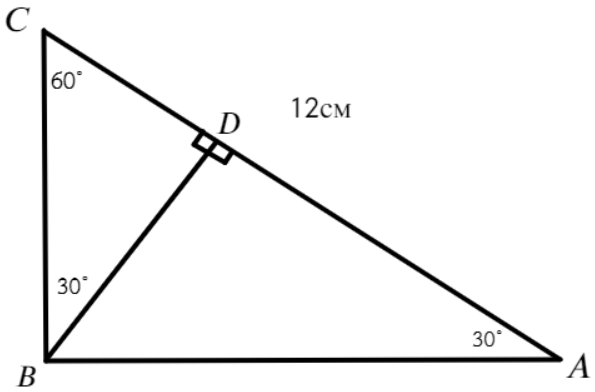
\includegraphics[scale=0.35]{g22.png}}
\end{figure}\\
$\angle C=90^\circ-\angle A=90^\circ-30^\circ=60^\circ,\ \angle CBD=90^\circ-\angle C=90^\circ-60^\circ=30^\circ.$ В прямоугольном треугольнике $ABC$ катет $BC$ лежит напротив угла в $30^\circ,$ а значит $BC=AC:2=12:2=6$см. В прямоугольном треугольнике $BCD$ катет $CD$ лежит напротив угла в $30^\circ,$ а значит $CD=BC:2=6:2=3$см. Тогда $DA=AC-CD=12-3=9$см.\\
